\section{Experiments}

\begin{table}[t]
  \centering
  \caption{Single-source retrieval comparison (accuracy \%). \textbf{Bold} = best in each row.}
  \label{tab:multisource_single}
  {\setlength{\tabcolsep}{4pt}
  \begin{tabular}{lccc}
    \toprule
    \textbf{Source} & \textbf{RAG} & \textbf{DA-Agent} & \textbf{Data2MCP} \\
    \midrule
    Spider   & 64.00 & 65.00 & \textbf{72.00} \\
    MetaQA   & 64.00 & \textbf{69.00} & 66.00 \\
    HotpotQA & 49.00 & 52.00 & \textbf{69.00} \\
    MS MARCO & 71.00 & 78.00 & \textbf{81.00} \\
    \cmidrule{1-4}
    Overall  & 62.00 & 66.00 & \textbf{72.00} \\
    \bottomrule
  \end{tabular}
  }
\end{table}

\begin{table*}[!t]
  \centering
  \caption{Multi-source retrieval comparison (accuracy \%). Strategy injection benefits both DA-Agent and Data2MCP. \textbf{Bold} = best in each column.}
  \label{tab:multisource_multi}
  {\setlength{\tabcolsep}{4pt}
  \begin{tabular*}{\textwidth}{@{\extracolsep{\fill}}lccccc}
    \toprule
    \textbf{System} & \textbf{Spider} & \textbf{MetaQA} & \textbf{HotpotQA} & \textbf{MS MARCO} & \textbf{Overall} \\
    \midrule
    \textit{Baselines} \\
    RAG                 & 49.00 & 54.00 & 43.00 & 59.00 & 51.25 \\
    DA-Agent            & 58.00 & 54.00 & 45.00 & 67.00 & 56.00 \\
    Data2MCP            & 62.00 & 52.00 & 57.00 & 67.00 & 59.50 \\
    \midrule
    \textit{DA-Agent + Strategy} \\
    + ACH               & 56.00 & 58.00 & 51.00 & 71.00 & 59.00 \\
    + CRISP-DM          & 63.00 & 59.00 & 55.00 & 64.00 & 60.25 \\
    + Auto-Select       & 62.00 & 61.00 & 52.00 & 70.00 & 61.25 \\
    + Adaptive          & 64.00 & 55.00 & 56.00 & 66.00 & 60.25 \\
    \midrule
    \textit{Data2MCP + Strategy} \\
    + ACH               & 65.00 & 54.00 & 61.00 & 70.00 & 62.50 \\
    + CRISP-DM          & 68.00 & 57.00 & 63.00 & 73.00 & 65.25 \\
    + Auto-Select       & \textbf{75.00} & 58.00 & 63.00 & \textbf{76.00} & 68.00 \\
    + Adaptive          & 70.00 & \textbf{62.00} & \textbf{67.00} & 75.00 & \textbf{68.50} \\
    \bottomrule
  \end{tabular*}
  }
\end{table*}

% \begin{figure*}[!t]
%   \centering
%   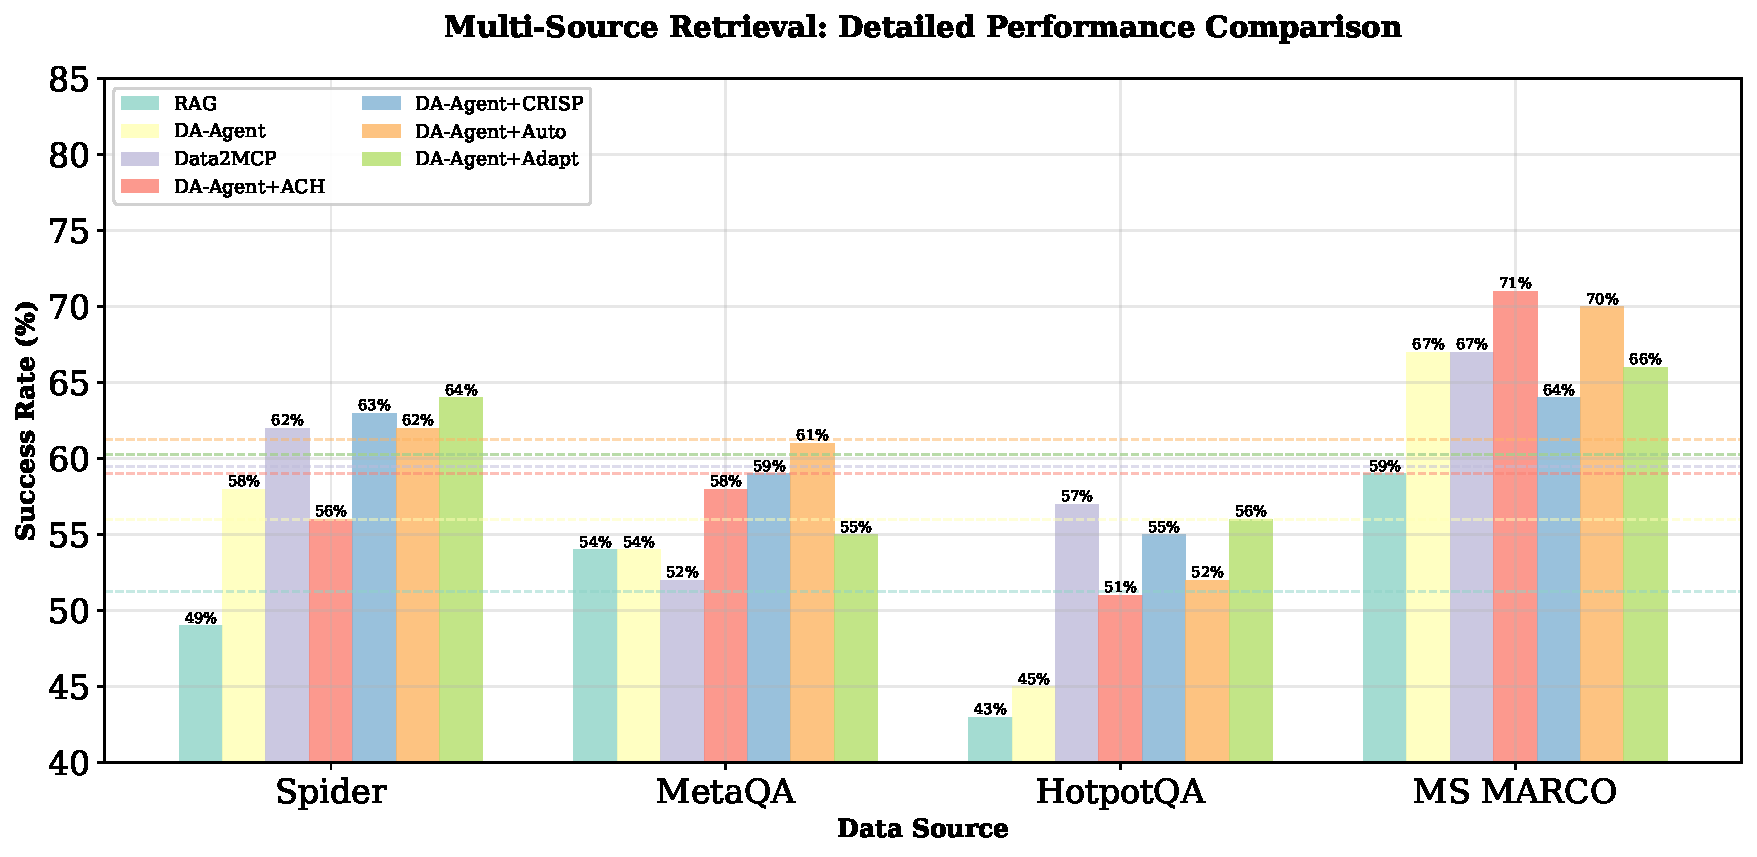
\includegraphics[width=1.0\textwidth]{figures/multisource_comparison_detailed.pdf}
%   \caption{Per-source breakdown of retrieval accuracy. Left: multi-source; middle: multi-source: Da-Agent + Strategy; right: multi-source: Data2MCP + Strategy.}
%   \label{fig:multisource_detailed}
% \end{figure*}


Our experiments address four research questions:

\begin{itemize}
  \item \textbf{RQ1}: Does Data2MCP's multi-source orchestration architecture
    effectively handle heterogeneous data retrieval compared to single-source
    specialized systems?
    (Section~\ref{sec:multisource})
  \item \textbf{RQ2}: Can frontier LLMs equipped with structured analytical
    methodologies achieve strong performance on complex data analysis tasks?
    (Section~\ref{sec:main})
  \item \textbf{RQ3}: Can an LLM autonomously discover effective analysis
    strategies by selecting from a catalog or generating bespoke strategies?
    (Section~\ref{sec:main}, Section~\ref{sec:analysis})
  \item \textbf{RQ4}: How do strategy-injected agents compare to other systems
    in analysis quality, stability, interpretability, and efficiency?
    (Section~\ref{sec:analysis}, Appendix~\ref{app:daagent})
\end{itemize}

\subsection{Benchmark, Evaluation, and Experimental Setup}

\paragraph{Multi-Source Retrieval experiment.}
For the multi-source retrieval experiments (Section~\ref{sec:multisource}), we evaluate both systems on 100 queries per data source (400 total) spanning four heterogeneous data sources: Spider~\cite{spider2018} (SQL), MetaQA~\cite{metaqa2018} (Knowledge Graph), HotpotQA~\cite{hotpotqa2018} (Elasticsearch), and MS MARCO~\cite{msmarco2016} (MongoDB). We test two scenarios: (1) Single-source: each query targets one data source; (2) Multi-source: each query requires synthesizing information from multiple sources. Success is measured by exact-match accuracy on ground-truth answers. We compare Data2MCP against DA-Agent and a baseline RAG system.

In this experiment, we use Qwen3-235B as the analysis agent for both Data2MCP and DA-Agent to keep the agent model fixed and reduce cross-provider evaluation artifacts. By fixing the agent model and evaluation protocol across systems, we isolate the impact of architectural choices and planning interventions (i.e., strategy injection) from model and scoring variance. We present the multi-source results first (RQ3) to directly validate Data2MCP's cross-source retrieval capability, and then return to DAComp (RQ1--RQ2) for end-to-end analysis.

\paragraph{DAComp experiment.}
We evaluate on DAComp~\cite{dacomp2025}, a benchmark of 100 heterogeneous data analysis tasks. Evaluation uses Gemini-2.5-Flash as the judge with three metric groups: Rubrics (60\% weight: Completeness, Accuracy, Conclusiveness), GSB-Text (20\% weight: Readability 10\%, Professionalism 10\%), and GSB-Visualization (20\% weight). Weighted total: $\text{Score} = 0.6 \!\times\! \text{Rubrics} + 0.1 \!\times\! \text{GSB\_Read} + 0.1 \!\times\! \text{GSB\_Prof} + 0.2 \!\times\! \text{GSB\_Vis}$.

In this experiment, we use GPT-5 as the analysis agent and Gemini-2.5-Flash as the judge for both Data2MCP and DA-Agent to keep the agent and evaluation protocols fixed across systems, while using a cross-provider judge to reduce same-provider bias. To account for run-to-run variability, we evaluate each configuration multiple times on the full 100-instance benchmark and report the average score (tables updated accordingly). Implementation details are provided in Appendix~\ref{app:impl}.


\subsection{Multi-Source Retrieval}
\label{sec:multisource}

Table~\ref{tab:multisource_single} and Table~\ref{tab:multisource_multi} compare Data2MCP, DA-Agent, and a RAG baseline under single-source and multi-source settings. Data2MCP outperforms DA-Agent in multi-source scenarios, reflecting the benefits of Router-based orchestration for cross-source evidence fusion. Figure~\ref{fig:multisource_overall} visualizes the overall breakdown.

\paragraph{Strategy Injection on Multi-Source Tasks.}
We evaluate strategy injection in the same setting. Table~\ref{tab:multisource_multi} presents the multi-source results for both DA-Agent + Strategy and Data2MCP + Strategy variants. Different strategies excel on different data sources (e.g., Auto-Select is strongest on Spider and MS MARCO, while Adaptive is best overall), motivating routing strategies based on task characteristics.

\begin{figure}[t]
  \centering
  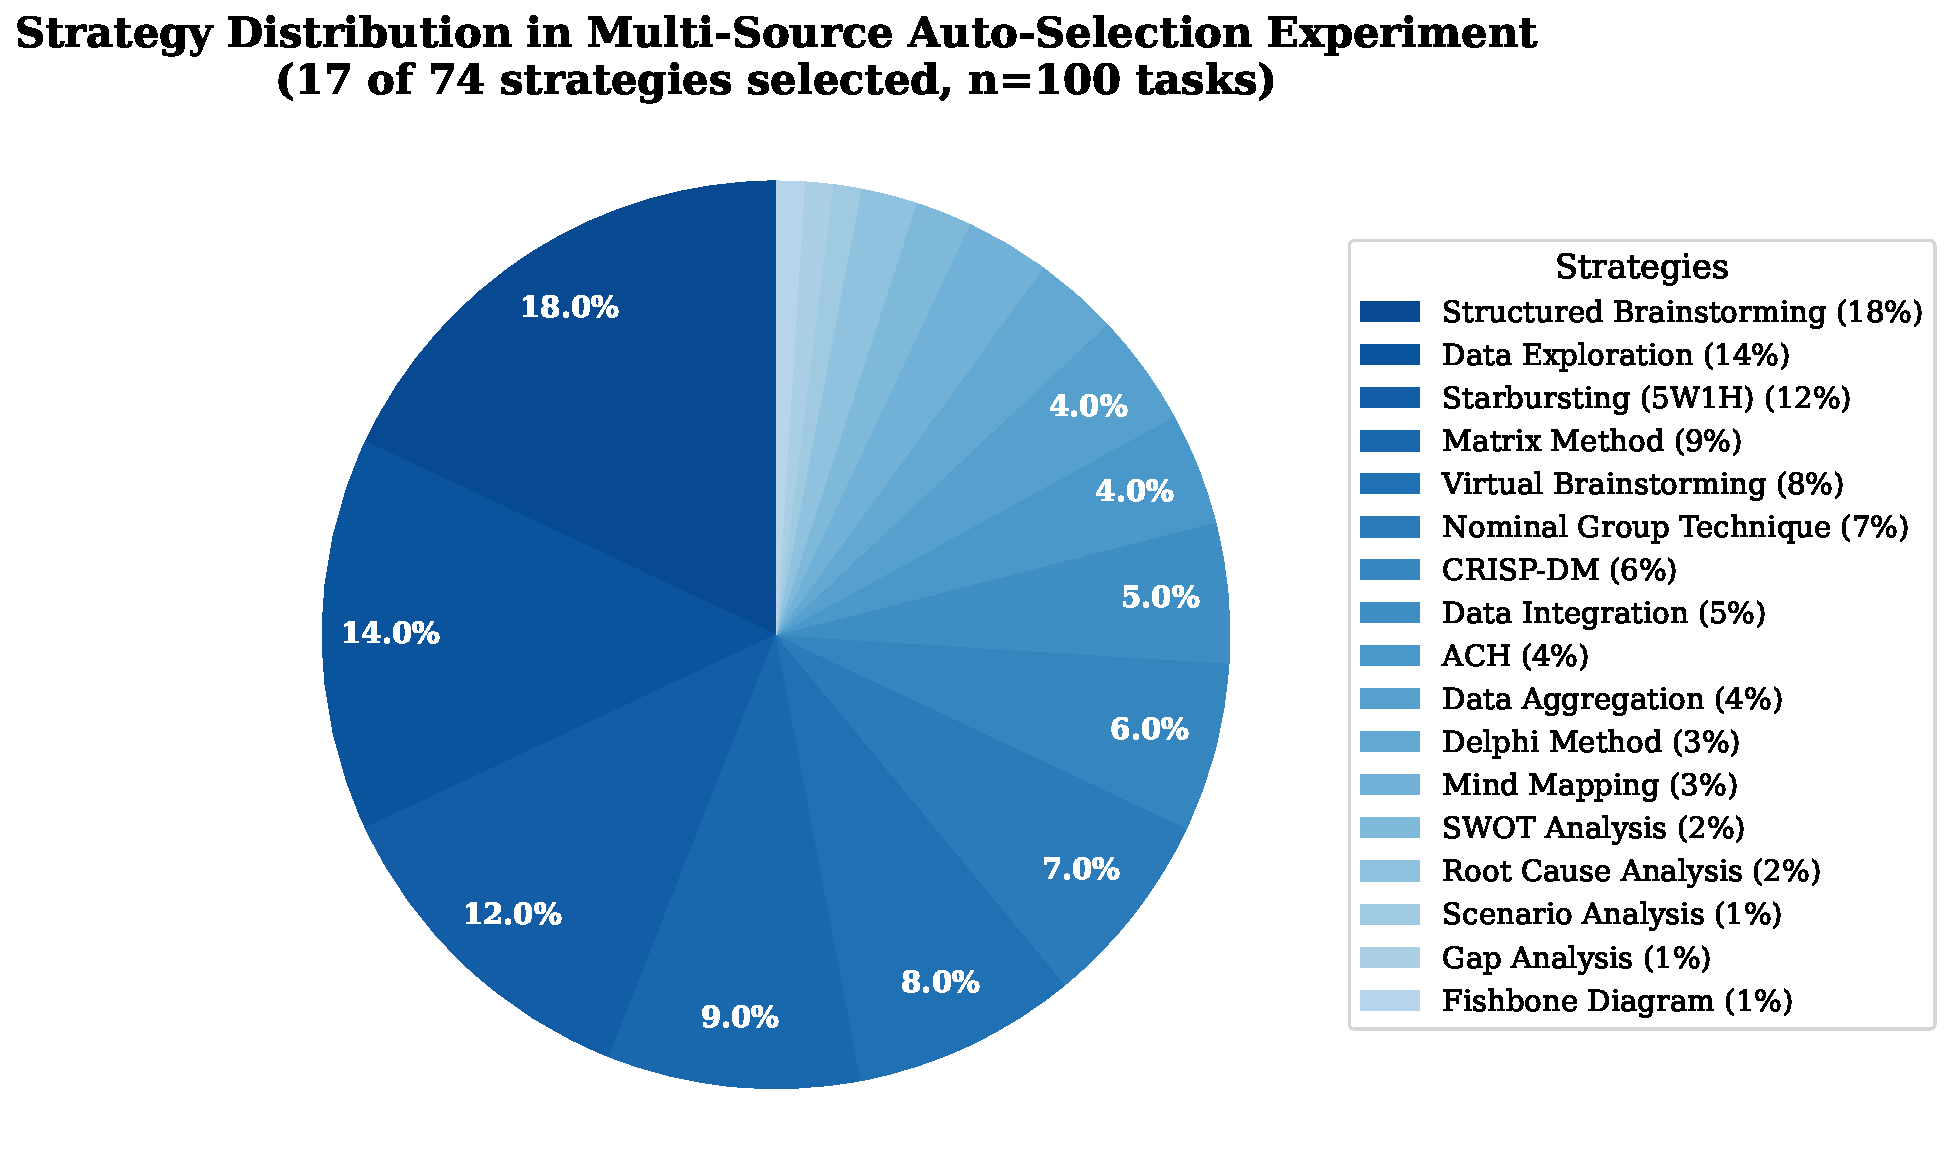
\includegraphics[width=\linewidth]{figures/multisource_strategy_distribution_pie.pdf}
  \caption{Strategy distribution in multi-source auto-selection experiment. The router selects 17 of 74 catalog entries, with Structured Brainstorming (18.0\%), Data Exploration (14.0\%), and Starbursting (12.0\%) as the top three strategies. This demonstrates strong task-awareness: compared to DAComp (where Data Exploration and Starbursting dominate), multi-source tasks favor Structured Brainstorming for parallel multi-source querying.}
  \label{fig:multisource_strategy_pie}
\end{figure}

\paragraph{Architectural Trade-offs.}
The gap in Table~\ref{tab:multisource_multi} reflects complementary design choices: Data2MCP emphasizes Router-based multi-agent orchestration (parallel cross-source tool selection, lightweight breadth-first queries, and MCP-standardized interfaces), which is well suited for heterogeneous retrieval and evidence fusion, whereas DA-Agent emphasizes depth-first single-source pipelines (EDA $\to$ modeling $\to$ visualization) with built-in analysis practices, which is better aligned with deep single-source analysis. Overall, these results suggest that architecture should match task breadth: router-based orchestration for heterogeneous retrieval and specialized pipelines for single-source analysis.


\begin{table*}[!t]
  \caption{Main results on DAComp. Agent: GPT-5. Judge: Gemini-2.5-Flash.
    All systems use the same agent and evaluation models for fair comparison.
    \textbf{Bold} = best in each system group.}
  \label{tab:main}
  \centering
  \setlength{\tabcolsep}{4pt}
  \begin{tabular*}{\textwidth}{@{\extracolsep{\fill}}lccccccc}
    \toprule
    \textbf{System} & \textbf{Comp.} & \textbf{Acc.} & \textbf{Conc.}
      & \textbf{GSB-R} & \textbf{GSB-P} & \textbf{GSB-V} & \textbf{W-Total} \\
    \midrule
    \multicolumn{8}{l}{\textit{Leaderboard baselines}} \\
    OpenHands        & 60.98 & 40.30 & 49.39 & 35.51 & 69.80 & 21.40 & 46.99 \\
    \midrule
    \multicolumn{8}{l}{\textit{Data2MCP}} \\
    No Strategy      & 55.45 & 38.76 & 53.06 & 34.89 & 65.78 & 26.39 & 46.40 \\
    + CRISP-DM       & 57.01 & 41.57 & 55.75 & 37.83 & 72.83 & 25.09 & 48.97 \\
    + ACH            & 59.15 & 39.98 & \textbf{55.06} & \textbf{44.74}
                     & \textbf{73.04} & 28.91 & \textbf{50.40} \\
    + Auto-Select    & \textbf{63.52} & 42.68 & 54.53 & 35.59 & 67.24
                     & 25.88 & 49.31 \\
    + Adaptive       & 61.75 & \textbf{44.65} & 57.03 & 34.27 & 64.24
                     & 22.55 & 48.83 \\
    \midrule
    \multicolumn{8}{l}{\textit{DA-Agent}} \\
    No Strategy      & 64.23 & 43.81 & 56.89 & 43.59 & 76.80 & 27.44 & 50.84 \\
    + CRISP-DM       & 65.87 & 46.23 & 59.34 & 45.67 & 80.31 & 30.18 & 52.92 \\
    + ACH            & 67.56 & 48.09 & \textbf{63.42} & 47.38 & \textbf{83.65}
                     & 31.47 & 55.21 \\
    + Auto-Select    & \textbf{71.28} & 51.64 & 62.39 & \textbf{49.73} & 83.12
                     & \textbf{33.76} & 57.10 \\
    + Adaptive       & 70.15 & \textbf{53.37} & 63.08 & 49.16 & 83.74
                     & 32.79 & \textbf{57.17} \\
    \bottomrule
  \end{tabular*}
\end{table*}



\begin{figure}[!t]
  \centering
  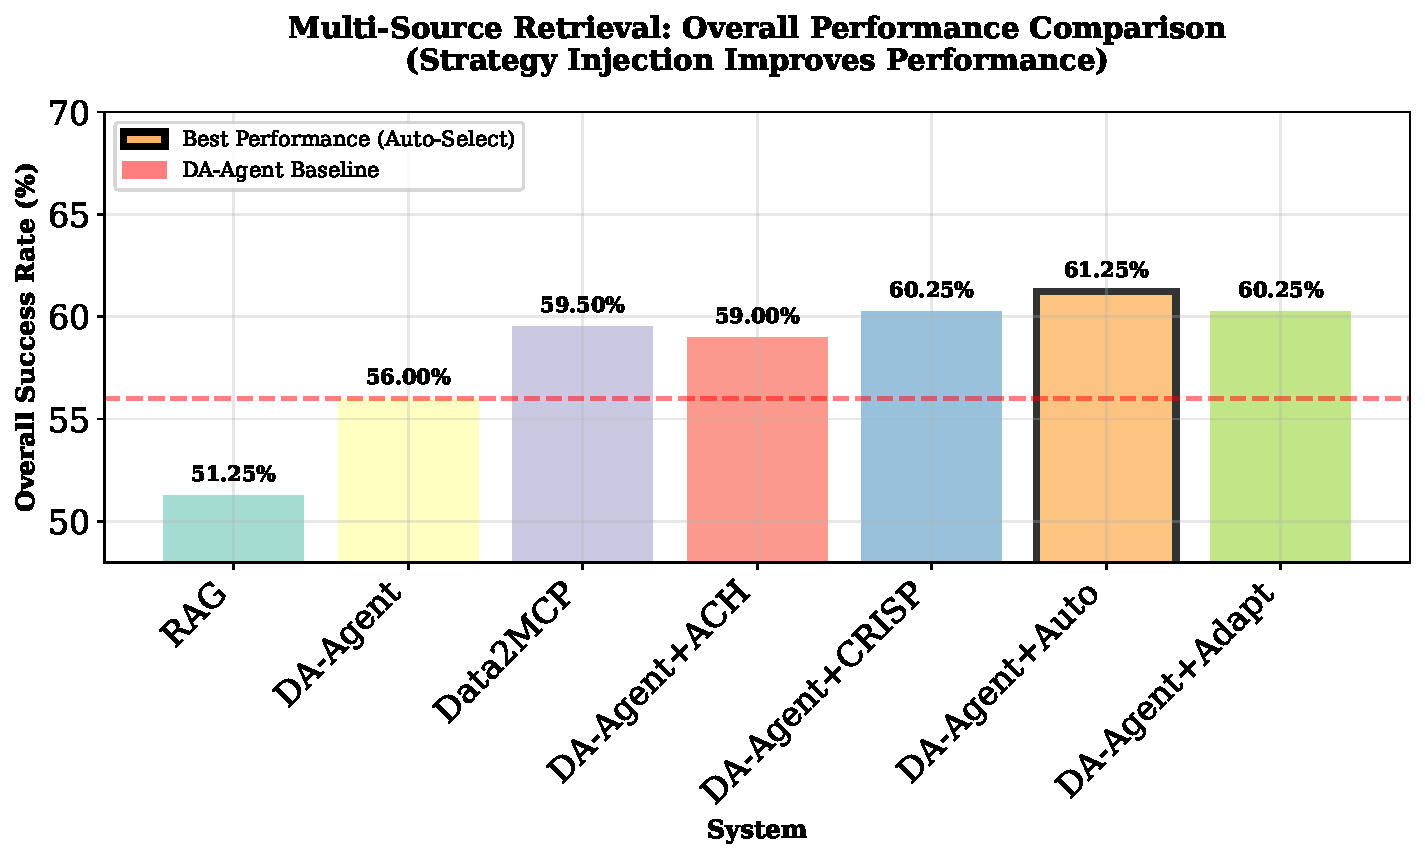
\includegraphics[width=\linewidth]{figures/multisource_comparison_overall.pdf}
  \caption{Multi-Source performance comparison between DA-Agent and DA-Agent + strategy.}
  \label{fig:multisource_overall}
\end{figure}

\subsection{DAComp: End-to-End Analysis Results with Strategy Injection}
\label{sec:main}

We now turn to DAComp (RQ1--RQ2), where each task requires end-to-end analysis and a coherent final report. We evaluate strategy injection on both Data2MCP and DA-Agent architectures to validate its effectiveness across different system designs. Table~\ref{tab:main} reports complete results for both architectures with GPT-5 as the analysis agent, evaluated by Gemini-2.5-Flash. Strategy injection consistently improves performance across both architectures, demonstrating the generality of our approach.



% \begin{figure*}[!t]
%   \centering
%   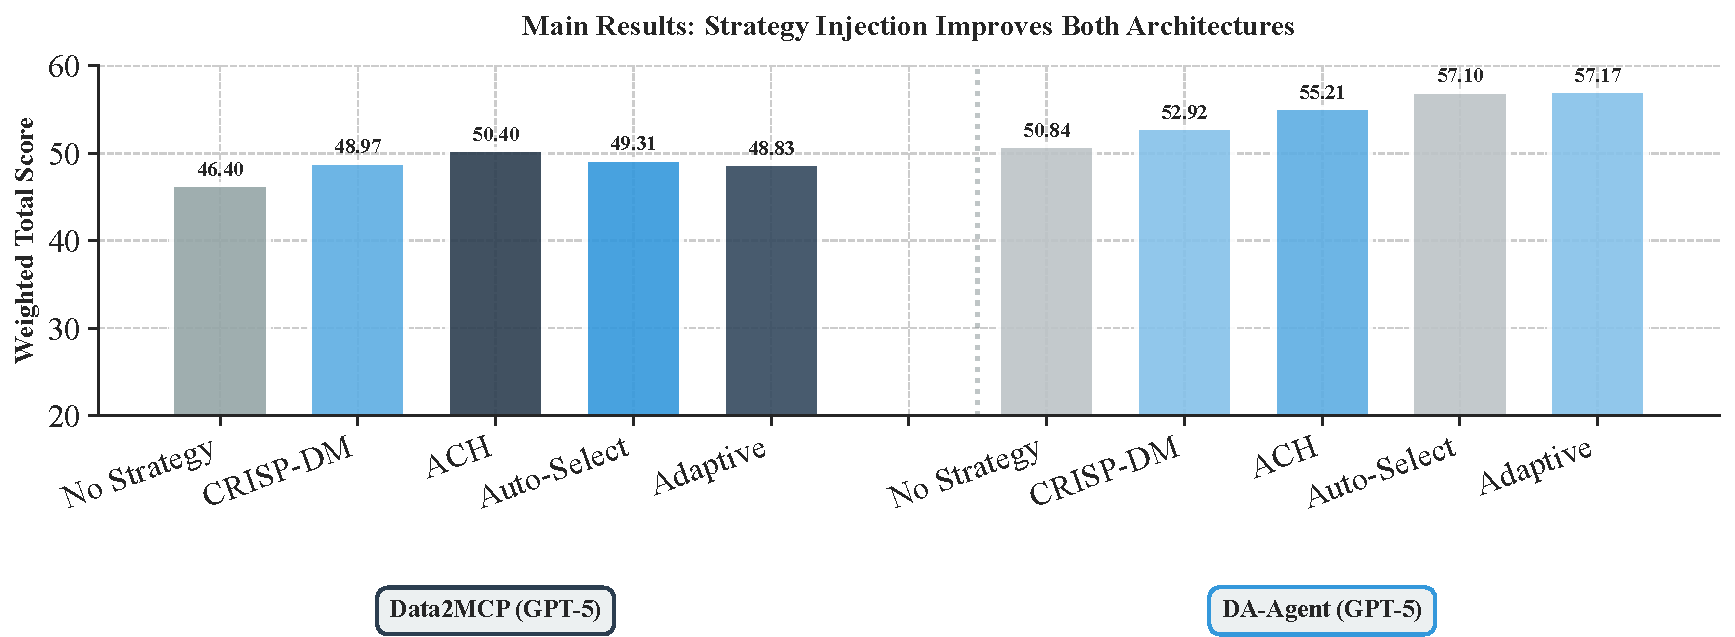
\includegraphics[width=0.98\textwidth]{figures/main_results_grouped_bar.pdf}
%   \caption{DAComp results: strategy injection improves both Data2MCP and DA-Agent. Deltas indicate gains over the No-Strategy baseline.}
%   \label{fig:main_results}
% \end{figure*}

\begin{figure}[t]
  \centering
  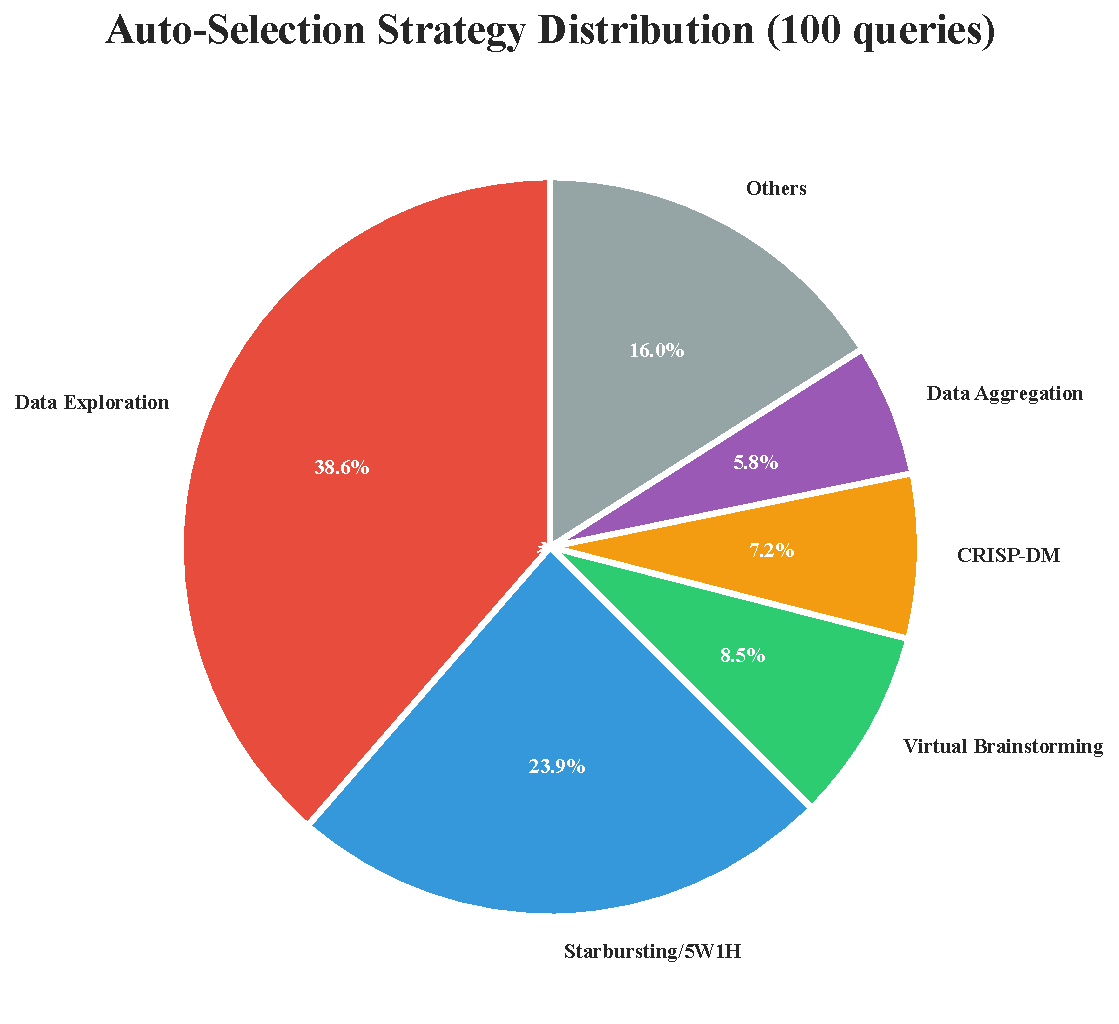
\includegraphics[width=\linewidth]{figures/strategy_distribution_pie.pdf}
  \caption{Strategy distribution of Auto-Select on the DAComp experiment. The router converges on 9 of 74 catalog entries, with Data Exploration (38.6\%) and Starbursting (23.9\%) covering 62.5\% of queries.}
  \label{fig:strategy_pie}
\end{figure}


\paragraph{Data2MCP Results.}
Strategy injection improves Data2MCP across all configurations, with the strongest gains coming from structured methodologies such as ACH. Different strategies exhibit complementary strengths: Auto-Select tends to increase coverage, Adaptive emphasizes correctness, and ACH improves conclusiveness and professional writing quality.

\paragraph{DA-Agent Results.}
DA-Agent also benefits from strategy injection, with Adaptive and Auto-Select performing best overall. Strategy-specific patterns mirror Data2MCP: Auto-Select improves completeness, Adaptive improves accuracy, and ACH improves conclusiveness and professionalism.

\paragraph{Cross-Architecture Observations.}
Overall, strategy injection provides consistent benefits across architectures, and strategy effects are largely stable: Auto-Select favors completeness, Adaptive favors accuracy, and ACH favors conclusiveness and professionalism. These results suggest that structured methodologies can partially compensate for architectural differences.

\subsection{Analysis}
\label{sec:analysis}

\paragraph{Which strategy works best and why?}
Results in Table~\ref{tab:main} suggest that structured methodologies (ACH, CRISP-DM) are most effective on end-to-end analytical tasks: they encourage explicit hypothesis testing, evidence-based writing, and clearer conclusions. In contrast, adaptive routing (Auto-Select) is most effective on heterogeneous multi-source retrieval, where the main challenge is selecting and combining evidence across sources.

\paragraph{Auto-selection routing behavior.}
The auto-selection router concentrates on a small subset of strategies rather than using the full catalog, indicating task-aware routing. On DAComp, it converges on 9 of 74 catalog entries (Figure~\ref{fig:strategy_pie}), dominated by Data Exploration (38.6\%) and Starbursting (23.9\%). On multi-source retrieval, it selects 17 of 74 entries with a flatter head (top strategy 18.0\%; Figure~\ref{fig:multisource_strategy_pie}), reflecting stronger diversity and a shift toward Structured Brainstorming for parallel cross-source querying. We also observe implicit quality filtering: many unused catalog entries are fine-grained workflow sub-steps (e.g., CRISP-DM stages) that are less reusable as high-level analytical playbooks. Finally, the selected strategies align with task types (e.g., trend/comparison queries map to Data Exploration, while causal/factor queries map to Starbursting), suggesting the router captures coarse-grained analytical intent.

These distributions provide direct evidence that the router can automatically adapt its methodological guidance to the query. Rather than relying on a single fixed playbook, Auto-Select identifies a small set of reusable strategies and shifts its preference across benchmarks (single-source DAComp vs. multi-source retrieval), which helps explain its consistent gains in Tables~\ref{tab:main} and \ref{tab:multisource_multi}.

\paragraph{Strategy injection mechanisms.}
Case studies (Appendix~\ref{app:cases}) highlight recurring mechanisms: stating objectives before querying, checking data quality, actively searching for contradictions, and ending with actionable recommendations.

\paragraph{Answering the research questions.}
Overall, strategy injection improves both architectures, and Auto-Select provides a practical way to adapt strategies to task characteristics. Detailed comparisons and extended analyses are provided in Appendix~\ref{app:daagent} and Appendix~\ref{app:analysis}.
